\chapter[Namelist options]{\hyperref[chap:namelist_sections]{Namelist options}}
\label{chap:namelist_tables}
Embedded links point to more detailed namelist information in the appendix.
\section[time\_management]{\hyperref[sec:nm_sec_time_management]{time\_management}}
\label{sec:nm_tab_time_management}
General time management is handled by the time\_management namelist record.
Included options handle time-related parts of MPAS, such as the calendar and if the simulation is a restart or not.

Users should use this record to specify the beginning time of the simulation,
and either the duration or the end of the simulation. Only the end or the
duration need to be specified as the other is derived within MPAS from the
beginning time and other specified one.

{\bf TBA: If both duration and stop are specified, then what happens?)}

{\small
\begin{center}
\begin{longtable}{| p{2.0in} || p{4.0in} |}
	\hline
	{\bf Name} & {\bf Description} \\
	\hline
	\hline
	\hyperref[subsec:nm_sec_config_do_restart]{config\_do\_restart} & Determines if the initial conditions should be read from a restart file, or an input file. \\
	\hline
	\hyperref[subsec:nm_sec_config_start_time]{config\_start\_time} & Timestamp describing the initial time of the simulation. If it is set to 'file', the initial time is read from restart\_timestamp. \\
	\hline
	\hyperref[subsec:nm_sec_config_stop_time]{config\_stop\_time} & Timestamp descriping the final time of the simulation. If it is set to 'none' the final time is determined from config\_start\_time and config\_run\_duration. \\
	\hline
	\hyperref[subsec:nm_sec_config_run_duration]{config\_run\_duration} & Timestamp describing the length of the simulation. If it is set to 'none' the duraction is determined from config\_start\_time and config\_stop\_time. config\_run\_duration overrides inconsistent values of config\_stop\_time. \\
	\hline
	\hyperref[subsec:nm_sec_config_calendar_type]{config\_calendar\_type} & Selection of the type of calendar that should be used in the simulation. \\
	\hline
\end{longtable}
\end{center}
}
\section[io]{\hyperref[sec:nm_sec_io]{io}}
\label{sec:nm_tab_io}
{\small
\begin{center}
\begin{longtable}{| p{2.0in} || p{4.0in} |}
	\hline
	{\bf Name} & {\bf Description} \\
	\hline
	\hline
	\hyperref[subsec:nm_sec_config_input_name]{config\_input\_name} & {\bf \color{red} MISSING} \\
	\hline
	\hyperref[subsec:nm_sec_config_output_name]{config\_output\_name} & {\bf \color{red} MISSING} \\
	\hline
	\hyperref[subsec:nm_sec_config_restart_name]{config\_restart\_name} & {\bf \color{red} MISSING} \\
	\hline
	\hyperref[subsec:nm_sec_config_restart_interval]{config\_restart\_interval} & {\bf \color{red} MISSING} \\
	\hline
	\hyperref[subsec:nm_sec_config_output_interval]{config\_output\_interval} & {\bf \color{red} MISSING} \\
	\hline
	\hyperref[subsec:nm_sec_config_stats_interval]{config\_stats\_interval} & {\bf \color{red} MISSING} \\
	\hline
	\hyperref[subsec:nm_sec_config_write_stats_on_startup]{config\_write\_stats\_on\_startup} & {\bf \color{red} MISSING} \\
	\hline
	\hyperref[subsec:nm_sec_config_write_output_on_startup]{config\_write\_output\_on\_startup} & {\bf \color{red} MISSING} \\
	\hline
	\hyperref[subsec:nm_sec_config_frames_per_outfile]{config\_frames\_per\_outfile} & {\bf \color{red} MISSING} \\
	\hline
	\hyperref[subsec:nm_sec_config_pio_num_iotasks]{config\_pio\_num\_iotasks} & {\bf \color{red} MISSING} \\
	\hline
	\hyperref[subsec:nm_sec_config_pio_stride]{config\_pio\_stride} & {\bf \color{red} MISSING} \\
	\hline
\end{longtable}
\end{center}
}
\section[time\_integration]{\hyperref[sec:nm_sec_time_integration]{time\_integration}}
\label{sec:nm_tab_time_integration}
The time integration namelist controls parameters that pertain to all time-stepping methods.  At present, Forward Euler is the only time integration method implemented.

{\small
\begin{center}
\begin{longtable}{| p{2.0in} || p{4.0in} |}
	\hline
	{\bf Name} & {\bf Description} \\
	\hline
	\hline
	\hyperref[subsec:nm_sec_config_dt]{config\_dt} & Length of model time-step. \\
	\hline
	\hyperref[subsec:nm_sec_config_time_integrator]{config\_time\_integrator} & Time integration method. \\
	\hline
\end{longtable}
\end{center}
}
\section[grid]{\hyperref[sec:nm_sec_grid]{grid}}
\label{sec:nm_tab_grid}
The grid namelist records provides options that modify both the horizontal and
vertical MPAS-Ocean grids. This namelist record can be used to modify the
number of halo cells each computational block contains, as well as changing how
vertical coordinates move.

{\small
\begin{center}
\begin{longtable}{| p{2.0in} || p{4.0in} |}
	\hline
	{\bf Name} & {\bf Description} \\
	\hline
	\hline
	\hyperref[subsec:nm_sec_config_num_halos]{config\_num\_halos} & Determines the number of halo cells extending from a blocks owned cells (Called the 0-Halo). The default of 3 is the minimum that can be used with monotonic advection. \\
	\hline
	\hyperref[subsec:nm_sec_config_vert_coord_movement]{config\_vert\_coord\_movement} & Determines the vertical coordinate movement type. 'uniform\_stretching' distrubtes SSH perturbations through all vertical levels, 'fixed' places them all in the top level, 'user\_specified' allows the input file to determine the distribution, and 'isopycnal' causes levels to be pure isopycnal. \\
	\hline
	\hyperref[subsec:nm_sec_config_alter_ICs_for_pbcs]{config\_alter\_ICs\_for\_pbcs} & Determines the method of alteration for partial bottom cells. 'zlevel\_pbcs\_on' alters the initial conditions for partial bottom cells, 'zlevel\_pbcs\_off' alters the initial conditions to have full cells everwhere, and 'off' does nothing to the initial conditions. \\
	\hline
	\hyperref[subsec:nm_sec_config_min_pbc_fraction]{config\_min\_pbc\_fraction} & Determines the minimum fraction of a cell altering the initial conditions can create. \\
	\hline
	\hyperref[subsec:nm_sec_config_check_ssh_consistency]{config\_check\_ssh\_consistency} & Enables a check to determine if the SSH is consistent across relevant variables. \\
	\hline
\end{longtable}
\end{center}
}
\section[decomposition]{\hyperref[sec:nm_sec_decomposition]{decomposition}}
\label{sec:nm_tab_decomposition}
MPAS handles decomposing all variables into computational blocks. The
decomposition used needs to be specified at run time and is computed by an
external tool (e.g. metis). Additionally, MPAS supports multiple computational
blocks per MPI process, and the user may specify an additional decomposition
file which can specify the assignment of blocks to MPI processes. Run-time
parameters that control the run-time decomposition used are specified within
the decomposition namelist record.


{\small
\begin{center}
\begin{longtable}{| p{2.0in} || p{4.0in} |}
	\hline
	{\bf Name} & {\bf Description} \\
	\hline
	\hline
	\hyperref[subsec:nm_sec_config_block_decomp_file_prefix]{config\_block\_decomp\_file\_prefix} & Defines the prefix for the block decomposition file. Can include a path. The number of blocks is appended to the end of the prefix at run-time. \\
	\hline
	\hyperref[subsec:nm_sec_config_number_of_blocks]{config\_number\_of\_blocks} & Determines the number of blocks a simulation should be run with. If it is set to 0, the number of blocks is the same as the number of MPI tasks at run-time. \\
	\hline
	\hyperref[subsec:nm_sec_config_explicit_proc_decomp]{config\_explicit\_proc\_decomp} & Determines if an explicit processor decomposition should be used. This is only useful if multiple blocks per processor are used. \\
	\hline
	\hyperref[subsec:nm_sec_config_proc_decomp_file_prefix]{config\_proc\_decomp\_file\_prefix} & Defines the prefix for the processor decomposition file. This file is only read if config\_explicit\_proc\_decomp is .true. The number of processors is appended to the end of the prefix at run-time. \\
	\hline
\end{longtable}
\end{center}
}
\section[hmix]{\hyperref[sec:nm_sec_hmix]{hmix}}
\label{sec:nm_tab_hmix}
There are several choices of horizontal mixing schemes available for the 
momentum and tracer equations.  Each of these is a turbulence closure, 
and attempts to account for subgrid-scale mixing and diffusion.  These 
schemes have the practical effect of reducing grid-scale noise in the 
velocity and tracer fields, and improving numerical stability.

Each horizontal mixing scheme has its own namelist, and may be turned
on with the \verb|_use_| logical configuration flags.  Multiple
schemes may be run simultaneously.  The horizontal mixing terms in the
governing equations (\ref{ocean:momentum},
\ref{ocean:tracer}) are ${\bf D}^u_h$ for momentum and
$D^\varphi_h$ for tracers.  No horizontal mixing is applied to the
thickness equation.

All horizontal mixing coefficients can be set to scale with the mesh as $\rho_m^{-3/4}$ in equations (\ref{ocean:\mode_h_mom_del2}, \ref{ocean:\mode_h_tr_del2}, \ref{ocean:\mode_h_mom_del4}, \ref{ocean:\mode_h_tr_del4}).  The mesh density, $\rho_m$, is a variable in the input and restart file.  It can vary between zero and one, and is one in the highest resolution region.  Scaling with the mesh can be turned off, as described in the options below.

The anticipated potential Vorticity (APV) method is a parameterization of the effects of subgrid or unresolved scales on those explicitly resolved \citep{Vallis_Hua88jas}.  It contributes an upstream bias to the vorticity in the del2 and del4 momentum terms as follows,
\begin{equation}
\eta_{apv} = \eta - c_{apv} dt \left({\bf u}\cdot \nabla \eta\right),
\end{equation}
where the altered vorticity $\eta_{apv}$ is used in equations (\ref{ocean:\mode_h_mom_del2}, \ref{ocean:\mode_h_mom_del4a}, \ref{ocean:\mode_h_mom_del4b}).

{\small
\begin{center}
\begin{longtable}{| p{2.0in} || p{4.0in} |}
	\hline
	{\bf Name} & {\bf Description} \\
	\hline
	\hline
	\hyperref[subsec:nm_sec_config_hmix_ScaleWithMesh]{config\_hmix\_ScaleWithMesh} &  If false, del2 and del4 coefficients are constant throughout the mesh (equivalent to setting  $\rho_m=1$  throughout the mesh).  If true, these coefficients scale as mesh density to the -3/4 power. \\
	\hline
	\hyperref[subsec:nm_sec_config_visc_vorticity_term]{config\_visc\_vorticity\_term} & {\color{red} TO BE DELETED} \\
	\hline
	\hyperref[subsec:nm_sec_config_apvm_scale_factor]{config\_apvm\_scale\_factor} &  Anticipated potential vorticity (APV) method scale factor,  $c_{apv}$ .  When zero, APV is off. \\
	\hline
\end{longtable}
\end{center}
}
\section[hmix\_del2]{\hyperref[sec:nm_sec_hmix_del2]{hmix\_del2}}
\label{sec:nm_tab_hmix_del2}
The ``del2'', or Laplacian, turbulence closures are
\begin{eqnarray}
\label{ocean:\mode_h_mom_del2}
& {\bf D}^u_h=\displaystyle\frac{\nu_h}{\rho_m^{3/4}} \nabla^2 {\bf u} 
= \displaystyle\frac{\nu_h}{\rho_m^{3/4}}(\nabla \delta + {\bf 
k}\times \nabla \eta),\\
\label{ocean:\mode_h_tr_del2}
& D^\varphi_h = \nabla\cdot\left(h 
   \displaystyle\frac{\kappa_h}{\rho_m^{3/4}} \nabla\varphi \right)
\end{eqnarray}
for momentum and tracers, respectively.  Variable definitions appear in Tables \ref{oceanTable:variables} and \ref{oceanTable:variables_Greek}.  The momentum diffusion is in divergence-vorticity form because it is a natural discretization of the vector Laplacian operator with a C-grid staggering.  

The Laplacian operator smooths the momentum and 
tracer fields, and smooths more strongly at small scales than at large 
scales.  This operator is the two dimensional form of the heat equation, 
$u_t=\nu u_{xx}$, described in introductory books on partial 
differential equations.  The strength of mixing is controlled by the 
viscosity, $\nu_h$, for the momentum equation, and the diffusion, 
$\kappa_h$, for the tracer equation.

{\small
\begin{center}
\begin{longtable}{| p{2.0in} || p{4.0in} |}
	\hline
	{\bf Name} & {\bf Description} \\
	\hline
	\hline
	\hyperref[subsec:nm_sec_config_use_mom_del2]{config\_use\_mom\_del2} & If true, Laplacian horizontal mixing is used on the momentum equation. \\
	\hline
	\hyperref[subsec:nm_sec_config_use_tracer_del2]{config\_use\_tracer\_del2} & If true, Laplacian horizontal mixing is used on the tracer equation. \\
	\hline
	\hyperref[subsec:nm_sec_config_mom_del2]{config\_mom\_del2} &  Horizonal viscosity,  $\nu_h$ . \\
	\hline
	\hyperref[subsec:nm_sec_config_tracer_del2]{config\_tracer\_del2} &  Horizonal diffusion,  $\kappa_h$ . \\
	\hline
	\hyperref[subsec:nm_sec_config_vorticity_del2_scale]{config\_vorticity\_del2\_scale} & {\color{red} TO BE DELETED} \\
	\hline
\end{longtable}
\end{center}
}
\section[hmix\_del4]{\hyperref[sec:nm_sec_hmix_del4]{hmix\_del4}}
\label{sec:nm_tab_hmix_del4}
The ``del4'', or biharmonic, turbulence closures are
\begin{eqnarray}
\label{ocean:\mode_h_mom_del4}
& {\bf D}^u_h=-\displaystyle\frac{\nu_h}{\rho_m^{3/4}} \nabla^4 {\bf u} \\
\label{ocean:\mode_h_tr_del4}
& D^\varphi_h = -\nabla\cdot\left(h \displaystyle\frac{\kappa_h}{\rho_m^{3/4}} \nabla \left[\nabla\cdot\left(h \nabla\varphi \right) \right] \right)
\end{eqnarray}
for momentum and tracers  These are both computed by applying the Laplacian operator twice.  For momentum, this can be written in terms of divergence and vorticity as
\begin{eqnarray}
&\delta=\nabla\cdot{\bf u}\\
&\eta={\bf k} \cdot \left( \nabla \times {\bf u} \right)+f\\
\label{ocean:\mode_h_mom_del4a}
&\nabla^2{\bf u}=(\nabla \delta + {\bf k}\times \nabla \eta) \\
&\delta_2=\nabla\cdot(\nabla^2{\bf u})\\
&\eta_2={\bf k} \cdot \left( \nabla \times (\nabla^2{\bf u}) \right)+f\\
\label{ocean:\mode_h_mom_del4b}
& {\bf D}^u_h= \displaystyle\frac{\nu_h}{\rho_m^{3/4}} (\nabla \delta_2 + {\bf k}\times \nabla \eta_2).
\end{eqnarray}
The biharmonic operator is similar to the Laplacian operator, but smooths more strongly at high wavenumbers.  

{\small
\begin{center}
\begin{longtable}{| p{2.0in} || p{4.0in} |}
	\hline
	{\bf Name} & {\bf Description} \\
	\hline
	\hline
	\hyperref[subsec:nm_sec_config_use_mom_del4]{config\_use\_mom\_del4} & If true, biharmonic horizontal mixing is used on the momentum equation. \\
	\hline
	\hyperref[subsec:nm_sec_config_use_tracer_del4]{config\_use\_tracer\_del4} & If true, biharmonic horizontal mixing is used on the tracer equation. \\
	\hline
	\hyperref[subsec:nm_sec_config_mom_del4]{config\_mom\_del4} & Coefficient for horizontal biharmonic operator on momentum. \\
	\hline
	\hyperref[subsec:nm_sec_config_tracer_del4]{config\_tracer\_del4} & Coefficient for horizontal biharmonic operator on tracers. \\
	\hline
	\hyperref[subsec:nm_sec_config_vorticity_del4_scale]{config\_vorticity\_del4\_scale} & {\color{red} TO BE DELETED} \\
	\hline
\end{longtable}
\end{center}
}
\section[hmix\_Leith]{\hyperref[sec:nm_sec_hmix_Leith]{hmix\_Leith}}
\label{sec:nm_tab_hmix_Leith}
The \cite{Leith:1996wu} closure is the enstrophy-cascade analogy to the \cite{Smagorinsky:1963wc} energy-cascade closure, i.e.  the Leith closure assumes an inertial range of enstrophy flux moving toward the grid scale. The assumption of an enstrophy cascade and dimensional analysis produces right-hand-side dissipation, $\bf{D}^u_h$, of velocity of the form

\begin{equation}
\label{eq:\mode_Leith}
{\bf D}^u_h =\nabla \cdot \left( \nu_h \nabla {\bf u} \right) = \nabla \cdot \left( \Gamma \left| \nabla \omega  \right| \left( \Delta x \right)^3 \nabla \bf{u} \right)
\end{equation}
where $\omega$ is the relative vorticity, ${\bf u}$ is the horizontal velocity, $\Delta x$ is the local grid spacing and $\Gamma$ is a non-dimensional, $O(1)$ parameter. This beta release approximates the RHS of the \ref{eq:Leith} as

\begin{equation}
\bf{D}^u_h=\nu_\ast \nabla_h^2 {\bf u}
\end{equation}
where the $\nabla^2 {\bf u}$ is computed using the form shown in \ref{ocean:\mode_h_mom_del4a}. Future releases will remove this approximation by computing the rate-of-strain, i.e. $\nabla {\bf u}$, directly.

{\small
\begin{center}
\begin{longtable}{| p{2.0in} || p{4.0in} |}
	\hline
	{\bf Name} & {\bf Description} \\
	\hline
	\hline
	\hyperref[subsec:nm_sec_config_use_Leith_del2]{config\_use\_Leith\_del2} & If true, the Leith enstrophy-cascade closure is turned on \\
	\hline
	\hyperref[subsec:nm_sec_config_Leith_parameter]{config\_Leith\_parameter} & Non-dimensional Leith closure parameter \\
	\hline
	\hyperref[subsec:nm_sec_config_Leith_dx]{config\_Leith\_dx} & Characteristic length scale, usually the smallest dx in the mesh \\
	\hline
	\hyperref[subsec:nm_sec_config_Leith_visc2_max]{config\_Leith\_visc2\_max} & Upper bound on the allowable value of Leith-computed viscosity \\
	\hline
\end{longtable}
\end{center}
}
\section[standard\_GM]{\hyperref[sec:nm_sec_standard_GM]{standard\_GM}}
\label{sec:nm_tab_standard_GM}
{\small
\begin{center}
\begin{longtable}{| p{2.0in} || p{4.0in} |}
	\hline
	{\bf Name} & {\bf Description} \\
	\hline
	\hline
	\hyperref[subsec:nm_sec_config_h_kappa]{config\_h\_kappa} & {\bf \color{red} MISSING} \\
	\hline
	\hyperref[subsec:nm_sec_config_h_kappa_q]{config\_h\_kappa\_q} & {\bf \color{red} MISSING} \\
	\hline
\end{longtable}
\end{center}
}
\section[Rayleigh\_damping]{\hyperref[sec:nm_sec_Rayleigh_damping]{Rayleigh\_damping}}
\label{sec:nm_tab_Rayleigh_damping}
A linear damping toward a state of rest is available with this namelist option.  It is implemented with a term on the RHS of the momentum equation (\ref{ocean:momentum}) of the form 
\begin{equation}
{\cal F}^u = -c_R {\bf u}.
\end{equation}


{\small
\begin{center}
\begin{longtable}{| p{2.0in} || p{4.0in} |}
	\hline
	{\bf Name} & {\bf Description} \\
	\hline
	\hline
	\hyperref[subsec:nm_sec_config_Rayleigh_friction]{config\_Rayleigh\_friction} & If true, Rayleigh friction is included in the momentum equation. \\
	\hline
	\hyperref[subsec:nm_sec_config_Rayleigh_damping_coeff]{config\_Rayleigh\_damping\_coeff} &  Inverse-time coefficient for the Rayleigh damping term,  $c_R$ . \\
	\hline
\end{longtable}
\end{center}
}
\section[vmix]{\hyperref[sec:nm_sec_vmix]{vmix}}
\label{sec:nm_tab_vmix}
{\small
\begin{center}
\begin{longtable}{| p{2.0in} || p{4.0in} |}
	\hline
	{\bf Name} & {\bf Description} \\
	\hline
	\hline
	\hyperref[subsec:nm_sec_config_convective_visc]{config\_convective\_visc} & {\bf \color{red} MISSING} \\
	\hline
	\hyperref[subsec:nm_sec_config_convective_diff]{config\_convective\_diff} & {\bf \color{red} MISSING} \\
	\hline
\end{longtable}
\end{center}
}
\section[vmix\_const]{\hyperref[sec:nm_sec_vmix_const]{vmix\_const}}
\label{sec:nm_tab_vmix_const}
{\small
\begin{center}
\begin{longtable}{| p{2.0in} || p{4.0in} |}
	\hline
	{\bf Name} & {\bf Description} \\
	\hline
	\hline
	\hyperref[subsec:nm_sec_config_use_const_visc]{config\_use\_const\_visc} & {\bf \color{red} MISSING} \\
	\hline
	\hyperref[subsec:nm_sec_config_use_const_diff]{config\_use\_const\_diff} & {\bf \color{red} MISSING} \\
	\hline
	\hyperref[subsec:nm_sec_config_vert_visc]{config\_vert\_visc} & {\bf \color{red} MISSING} \\
	\hline
	\hyperref[subsec:nm_sec_config_vert_diff]{config\_vert\_diff} & {\bf \color{red} MISSING} \\
	\hline
\end{longtable}
\end{center}
}
\section[vmix\_rich]{\hyperref[sec:nm_sec_vmix_rich]{vmix\_rich}}
\label{sec:nm_tab_vmix_rich}
{\small
\begin{center}
\begin{longtable}{| p{2.0in} || p{4.0in} |}
	\hline
	{\bf Name} & {\bf Description} \\
	\hline
	\hline
	\hyperref[subsec:nm_sec_config_use_rich_visc]{config\_use\_rich\_visc} & {\bf \color{red} MISSING} \\
	\hline
	\hyperref[subsec:nm_sec_config_use_rich_diff]{config\_use\_rich\_diff} & {\bf \color{red} MISSING} \\
	\hline
	\hyperref[subsec:nm_sec_config_bkrd_vert_visc]{config\_bkrd\_vert\_visc} & {\bf \color{red} MISSING} \\
	\hline
	\hyperref[subsec:nm_sec_config_bkrd_vert_diff]{config\_bkrd\_vert\_diff} & {\bf \color{red} MISSING} \\
	\hline
	\hyperref[subsec:nm_sec_config_rich_mix]{config\_rich\_mix} & {\bf \color{red} MISSING} \\
	\hline
\end{longtable}
\end{center}
}
\section[vmix\_tanh]{\hyperref[sec:nm_sec_vmix_tanh]{vmix\_tanh}}
\label{sec:nm_tab_vmix_tanh}
{\small
\begin{center}
\begin{longtable}{| p{2.0in} || p{4.0in} |}
	\hline
	{\bf Name} & {\bf Description} \\
	\hline
	\hline
	\hyperref[subsec:nm_sec_config_use_tanh_visc]{config\_use\_tanh\_visc} & {\bf \color{red} MISSING} \\
	\hline
	\hyperref[subsec:nm_sec_config_use_tanh_diff]{config\_use\_tanh\_diff} & {\bf \color{red} MISSING} \\
	\hline
	\hyperref[subsec:nm_sec_config_max_visc_tanh]{config\_max\_visc\_tanh} & {\bf \color{red} MISSING} \\
	\hline
	\hyperref[subsec:nm_sec_config_min_visc_tanh]{config\_min\_visc\_tanh} & {\bf \color{red} MISSING} \\
	\hline
	\hyperref[subsec:nm_sec_config_max_diff_tanh]{config\_max\_diff\_tanh} & {\bf \color{red} MISSING} \\
	\hline
	\hyperref[subsec:nm_sec_config_min_diff_tanh]{config\_min\_diff\_tanh} & {\bf \color{red} MISSING} \\
	\hline
	\hyperref[subsec:nm_sec_config_zMid_tanh]{config\_zMid\_tanh} & {\bf \color{red} MISSING} \\
	\hline
	\hyperref[subsec:nm_sec_config_zWidth_tanh]{config\_zWidth\_tanh} & {\bf \color{red} MISSING} \\
	\hline
\end{longtable}
\end{center}
}
\section[forcing]{\hyperref[sec:nm_sec_forcing]{forcing}}
\label{sec:nm_tab_forcing}
Namelist parameters for the \verb+forcing+ namelist group.

{\small
\begin{center}
\begin{longtable}{| p{2.0in} || p{4.0in} |}
	\hline
	{\bf Name} & {\bf Description} \\
	\hline
	\hline
	\hyperref[subsec:nm_sec_config_use_monthly_forcing]{config\_use\_monthly\_forcing} & Controls time frequency of forcing.  If false, a constant forcing is used, provided by the input fields normalVelocityForcing, temperatureRestore, and salinityRestore.  If true, forcing is interpolated between monthly fields given by windStressMonthly, temperatureRestoreMonthly, and salinityRestoreMonthly. \\
	\hline
	\hyperref[subsec:nm_sec_config_restoreTS]{config\_restoreTS} & If true, the restoring term is activated in the tracer equation for temperature and salinity. \\
	\hline
	\hyperref[subsec:nm_sec_config_restoreT_timescale]{config\_restoreT\_timescale} &  Restoring timescale for temperature,  $\tau_r.$  \\
	\hline
	\hyperref[subsec:nm_sec_config_restoreS_timescale]{config\_restoreS\_timescale} &  Restoring timescale for salinity,  $\tau_r$ . \\
	\hline
\end{longtable}
\end{center}
}
\section[advection]{\hyperref[sec:nm_sec_advection]{advection}}
\label{sec:nm_tab_advection}
The advection namelist record controls options assocated with advection of thickness and tracers.  Tracer advection is not currently supported.

{\small
\begin{center}
\begin{longtable}{| p{2.0in} || p{4.0in} |}
	\hline
	{\bf Name} & {\bf Description} \\
	\hline
	\hline
	\hyperref[subsec:nm_sec_config_vert_tracer_adv]{config\_vert\_tracer\_adv} & Method for interpolating tracer values from layer centers to layer edges \\
	\hline
	\hyperref[subsec:nm_sec_config_vert_tracer_adv_order]{config\_vert\_tracer\_adv\_order} & Order of polynomial used for tracer reconstruction at layer edges \\
	\hline
	\hyperref[subsec:nm_sec_config_horiz_tracer_adv_order]{config\_horiz\_tracer\_adv\_order} & Order of polynomial used for tracer reconstruction at cell edges \\
	\hline
	\hyperref[subsec:nm_sec_config_coef_3rd_order]{config\_coef\_3rd\_order} & Reconstruction of 3rd-order reconstruction to blend with 4th-order reconstuction \\
	\hline
	\hyperref[subsec:nm_sec_config_monotonic]{config\_monotonic} & If .true. then fluxes are limited to produce a monotonic advection scheme \\
	\hline
\end{longtable}
\end{center}
}
\section[bottom\_drag]{\hyperref[sec:nm_sec_bottom_drag]{bottom\_drag}}
\label{sec:nm_tab_bottom_drag}
The bottom drag is applied as a bottom boundary condition within the implicit solve of vertical mixing in the momentum equation (\ref{ocean:momentum}), as
\begin{equation}
\lim_{z\rightarrow z_{bot}} \nu_v \frac{\partial u}{\partial z} = c_{drag} \left|u\right| u,
\end{equation}
where $c_{drag}$ is the dimensionless bottom drag coefficient, and $z_{bot}$ is the $z$-location of the ocean bottom.

{\small
\begin{center}
\begin{longtable}{| p{2.0in} || p{4.0in} |}
	\hline
	{\bf Name} & {\bf Description} \\
	\hline
	\hline
	\hyperref[subsec:nm_sec_config_bottom_drag_coeff]{config\_bottom\_drag\_coeff} &  Dimensionless bottom drag coefficient,  $c_{drag}$ . \\
	\hline
\end{longtable}
\end{center}
}
\section[pressure\_gradient]{\hyperref[sec:nm_sec_pressure_gradient]{pressure\_gradient}}
\label{sec:nm_tab_pressure_gradient}
There are several formulations for the pressure gradient.
 
{\bf \large config\_pressure\_gradient\_type = 'pressure\_and\_zmid'}\\
This is the standard setting, and may be used for most configurations.  Here the pressure gradient terms in the momentum equation will have the form
\begin{equation}
\label{ocean:grad p}
- \frac{1}{\rho_0}\nabla_z p = - \frac{1}{\rho_0}\nabla_s p - \frac{\rho g}{\rho_0}\nabla_s z^{mid}.
\end{equation}
where $\nabla_z$ is the horizonal gradient along a constant $z$ surface and $\nabla_s$ is the gradient along a layer, which is a natural way to compute horizontal derivatives within the model.  Note that if a layer's depth is constant in the horizontal, then the second term is zero.

\begin{figure}[htb]
\centering
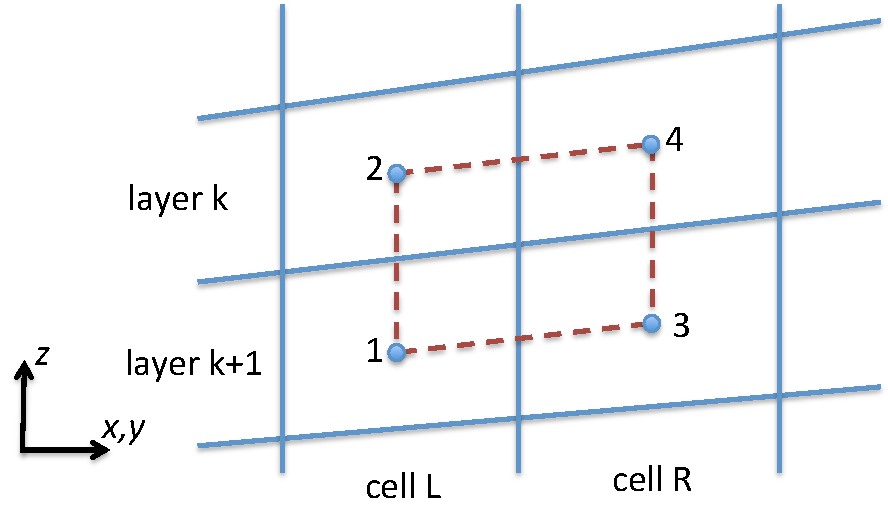
\includegraphics[width=3.5in]{ocean/figures/common_level.pdf}
\caption{Vertical cross-section of ocean grid cells, showing index locations for common level method.  The dots are placed at cell centers in the horizontal and layer mid-depth in the vertical.}
\label{oceanFigure:common level}
\end{figure}

{\bf \large config\_pressure\_gradient\_type = 'Jacobian\_from\_density'}\\
In this formulation the pressure gradient is rewritten in terms of a sea surface height gradient and the vertical integral of a Jacobian,
\begin{eqnarray}
\label{ocean:grad p Jacobian}
- \frac{1}{\rho_0}\nabla_z p &=& - \frac{\rho_s g}{\rho_0}\nabla_s \zeta - \frac{g}{\rho_0}\int_z^\zeta {\mathcal J}(\rho,z)ds, \\
{\mathcal J}(\rho,z) &=& \left. \frac{\partial \rho}{\partial x} \right|_s \frac{\partial z}{\partial s} 
 - \frac{\partial \rho}{\partial s}  \left. \frac{\partial z}{\partial x} \right|_s 
\end{eqnarray}
where $x$ is a general horizontal direction between two cell centers and $s$ is the vertical coordinate reference, i.e.\ $s$ is constant within a layer.  There are many methods to discretize the Jacobian term.  In the common level method, the density is linearly interpolated or extrapolated within each vertical column to a common level $z_\gamma$ (see Figure \ref{oceanFigure:common level}):
\begin{eqnarray}
- \int_z^\zeta {\mathcal J}(\rho,z)ds &=& \overline{\Delta z} \left( \rho^L - \rho^R \right) \\
\overline{\Delta z} &=& \frac{1}{2} \left(z_2-z_1 + z_4-z_3\right) \\
\rho^L &=& \frac{\rho_1\left(z_2-z_\gamma\right) + \rho_2\left(z_\gamma-z_1\right) }{z_2-z_1}\\
\rho^R &=& \frac{\rho_3\left(z_4-z_\gamma\right) + \rho_4\left(z_\gamma-z_3\right) }{z_4-z_3}\\
z_\gamma &=& \left(1-\gamma\right)z_* + \gamma z_c \\
z_* &=&  \frac{z_4 z_2-z_3z_1}{z_4-z_3 + z_2-z_1} \\
z_c &=&  \frac{z_1+z_2+z_3+z_4}{4} 
\end{eqnarray}
where $z_c$ is the depth for the weighted Jacobian method by \citet{Song98mwr}, and $z_*$ is the depth for the standard Jacobian method, which is the depth of intersection of the diagonals of the trapezoidal element in Figure \ref{oceanFigure:common level}.  Here $\gamma$ weights the choice between these two methods for computing the common level $z_\gamma$.  This formulation for the pressure gradient is described in detail in \citet{Shchepetkin_McWilliams03jgr}, Section 2, method 2, and Section 4.  They found that a coefficient of $\gamma=0.5$, which gives equal weights to the standard and weighted Jacobian methods, minimizes the errors in a seamount test problem.

{\bf \large config\_pressure\_gradient\_type = 'Jacobian\_from\_TS'}\\
This formulation is the same as the previous, except that the Jacobian is computed using a linear expansion in potential temperature and salinity.  This option must be used when layers are extremely tilted, such as with sigma coordinates or under an ice shelf, in combination with a nonlinear equation of state.
\begin{eqnarray}
 {\mathcal J}(\rho,z) &=& -\alpha  {\mathcal J}(\theta,z) + \beta  {\mathcal J}(S,z), 
\end{eqnarray}
where
\begin{eqnarray}
\alpha\left( \theta, S, p\right) &=&  -\left. \frac{\partial \rho}{\partial \theta} \right|_{S,p} \\
\beta\left( \theta, S, p\right) &=&  \left. \frac{\partial \rho}{\partial S} \right|_{\theta,p} 
\end{eqnarray}
are the thermal expansion and saline contraction coefficients, computed at a particular  $\left(\theta, S, p\right)$ by the equation of state \citep[eqn 7.16]{Shchepetkin_McWilliams03jgr}.

{\bf \large config\_pressure\_gradient\_type = 'MontgomeryPotential'}\\
For isopycnal vertical coordinates, the user may choose to use the Montgomery potential,
\begin{equation}
\label{ocean:Montgomery Potential}
M = \frac{1}{\rho}p+gz
\end{equation}
and replace the pressure terms above with
\begin{equation}
- \nabla_s M.
\end{equation}
See \citet[section 2.1]{Higdon05jcp} for details on the derivation and computation of the Montgomery potential.

% {\bf \large config\_pressure\_gradient\_type = 'MontgomeryPotential\_and\_density'}
% Same as previous, but this formulation includes an extra term,
% \begin{equation}
% - \nabla_s M + p \nabla_s\left(\frac{1}{\rho} \right),
% \end{equation}
% as described by \citet{Bleck02om}, eqn 1 and end of Appendix A.  This formulation has not been extensively tested and is not supported at this time.

{\small
\begin{center}
\begin{longtable}{| p{2.0in} || p{4.0in} |}
	\hline
	{\bf Name} & {\bf Description} \\
	\hline
	\hline
	\hyperref[subsec:nm_sec_config_pressure_gradient_type]{config\_pressure\_gradient\_type} & Form of pressure gradient terms in momentum equation. For most applications, the gradient of pressure and layer mid-depth are appropriate.  For isopycnal coordinates, one may use the gradient of the Montgomery potential. \\
	\hline
	\hyperref[subsec:nm_sec_config_density0]{config\_density0} &  Density used as a coefficient of the pressure gradient terms,  $\rho_0$ .  This is a constant due to the Boussinesq approximation. \\
	\hline
\end{longtable}
\end{center}
}
\section[eos]{\hyperref[sec:nm_sec_eos]{eos}}
\label{sec:nm_tab_eos}
Two forms of EOS are supported. The full EOS from \cite{Jackett_McDougall95jaot} and a linear EOS.

{\small
\begin{center}
\begin{longtable}{| p{2.0in} || p{4.0in} |}
	\hline
	{\bf Name} & {\bf Description} \\
	\hline
	\hline
	\hyperref[subsec:nm_sec_config_eos_type]{config\_eos\_type} & Character string to choose EOS formulation \\
	\hline
\end{longtable}
\end{center}
}
\section[eos\_linear]{\hyperref[sec:nm_sec_eos_linear]{eos\_linear}}
\label{sec:nm_tab_eos_linear}
The linear equation of state (leos) is specified as follows:
\begin{equation}
\rho = \rho_{ref} - \alpha_{leos}(T-T_{ref})+\beta_{leos}(S-S_{ref})
\end{equation}
{\small
\begin{center}
\begin{longtable}{| p{2.0in} || p{4.0in} |}
	\hline
	{\bf Name} & {\bf Description} \\
	\hline
	\hline
	\hyperref[subsec:nm_sec_config_eos_linear_alpha]{config\_eos\_linear\_alpha} & Linear thermal expansion coefficient \\
	\hline
	\hyperref[subsec:nm_sec_config_eos_linear_beta]{config\_eos\_linear\_beta} & Linear haline contraction coefficient \\
	\hline
	\hyperref[subsec:nm_sec_config_eos_linear_Tref]{config\_eos\_linear\_Tref} & Reference temperature \\
	\hline
	\hyperref[subsec:nm_sec_config_eos_linear_Sref]{config\_eos\_linear\_Sref} & Reference salinity \\
	\hline
	\hyperref[subsec:nm_sec_config_eos_linear_densityref]{config\_eos\_linear\_densityref} & Reference density, i.e. density when T=Tref and S=Sref \\
	\hline
\end{longtable}
\end{center}
}
\section[split\_explicit\_ts]{\hyperref[sec:nm_sec_split_explicit_ts]{split\_explicit\_ts}}
\label{sec:nm_tab_split_explicit_ts}
The split explicit time-stepping method solves the barotropic (vertically-integrated) velocities separately from the remaining baroclinic velocities.  The time step for the barotropic solve is limited by fast surface gravity waves, and so is subcycled within a large timestep of the baroclinic velocity solve.  This provides a 10 to 12-times speed-up over fourth-order Runge-Kutta time stepping.

A single large timestep in the split explicit algorithm may be summarized as
\begin{itemize}
\item Stage 1: solve for baroclinic velocity (3D)
\item Stage 2: solve for barotropic velocity (2D) with explicit sub-cycling
\item Stage 3: update thickness, tracers, density and pressure
\end{itemize}
The algorithm includes iterations within stage 1, within each subcycle of stage 2, and over the full three-stage process.  Further details are provided in \citet[Appendix A.5]{Ringler_ea13om}

{\small
\begin{center}
\begin{longtable}{| p{2.0in} || p{4.0in} |}
	\hline
	{\bf Name} & {\bf Description} \\
	\hline
	\hline
	\hyperref[subsec:nm_sec_config_n_ts_iter]{config\_n\_ts\_iter} & number of large iterations over stages 1-3 \\
	\hline
	\hyperref[subsec:nm_sec_config_n_bcl_iter_beg]{config\_n\_bcl\_iter\_beg} & number of iterations of stage 1 (baroclinic solve) on the first split-explicit iteration \\
	\hline
	\hyperref[subsec:nm_sec_config_n_bcl_iter_mid]{config\_n\_bcl\_iter\_mid} & number of iterations of stage 1 (baroclinic solve) on any split-explicit iterations between first and last \\
	\hline
	\hyperref[subsec:nm_sec_config_n_bcl_iter_end]{config\_n\_bcl\_iter\_end} & number of iterations of stage 1 (baroclinic solve) on the last split-explicit iteration \\
	\hline
	\hyperref[subsec:nm_sec_config_n_btr_subcycles]{config\_n\_btr\_subcycles} & number of barotropic subcycles in stage 2 \\
	\hline
	\hyperref[subsec:nm_sec_config_n_btr_cor_iter]{config\_n\_btr\_cor\_iter} & number of iterations of the velocity corrector step in stage 2 \\
	\hline
	\hyperref[subsec:nm_sec_config_vel_correction]{config\_vel\_correction} & If true, the velocity correction term is included in the horizontal advection of thickness and tracers \\
	\hline
	\hyperref[subsec:nm_sec_config_btr_subcycle_loop_factor]{config\_btr\_subcycle\_loop\_factor} &  Barotropic subcycles proceed from  $t$  to  $t+n\Delta t$ , where  $n$  is this configuration option. \\
	\hline
	\hyperref[subsec:nm_sec_config_btr_gam1_velWt1]{config\_btr\_gam1\_velWt1} & Weighting of velocity in the SSH predictor step in stage 2.  When zero, previous subcycle time is used; when one, new subcycle time is used. \\
	\hline
	\hyperref[subsec:nm_sec_config_btr_gam2_SSHWt1]{config\_btr\_gam2\_SSHWt1} & Weighting of SSH in the velocity corrector step in stage 2.  When zero, previous subcycle time is used; when one, new subcycle time is used. \\
	\hline
	\hyperref[subsec:nm_sec_config_btr_gam3_velWt2]{config\_btr\_gam3\_velWt2} & Weighting of velocity in the SSH corrector step in stage 2.  When zero, previous subcycle time is used; when one, new subcycle time is used. \\
	\hline
	\hyperref[subsec:nm_sec_config_btr_solve_SSH2]{config\_btr\_solve\_SSH2} & If true, execute the SSH corrector step in stage 2 \\
	\hline
\end{longtable}
\end{center}
}
\section[debug]{\hyperref[sec:nm_sec_debug]{debug}}
\label{sec:nm_tab_debug}
At run-time a user can enable debugging features within MPAS-Ocean. These
features include disabling any tendencies to help determine why an issue might
be happening. Debugging options also include various checks on certain fields,
and the ability to prescribe both a thickness and velocity field at run-time
which are constant throughout a simulation. All options that control these
debugging features are specified within the debug namelist record.

{\small
\begin{center}
\begin{longtable}{| p{2.0in} || p{4.0in} |}
	\hline
	{\bf Name} & {\bf Description} \\
	\hline
	\hline
	\hyperref[subsec:nm_sec_config_check_zlevel_consistency]{config\_check\_zlevel\_consistency} & Enables a run-time check for consistency for a zlevel grid. Ensures relevant variables correctly define the bottom of the ocean. \\
	\hline
	\hyperref[subsec:nm_sec_config_filter_btr_mode]{config\_filter\_btr\_mode} & Enables filtering of the barotropic mode. \\
	\hline
	\hyperref[subsec:nm_sec_config_prescribe_velocity]{config\_prescribe\_velocity} & Enables a prescribed velocity field. This velocity field is read on input, and remains constant through a simulation. \\
	\hline
	\hyperref[subsec:nm_sec_config_prescribe_thickness]{config\_prescribe\_thickness} & Enables a prescribed thickness field. This thickness field is read on input, and remains constant through a simulation. \\
	\hline
	\hyperref[subsec:nm_sec_config_include_KE_vertex]{config\_include\_KE\_vertex} & {\bf \color{red} MISSING} \\
	\hline
	\hyperref[subsec:nm_sec_config_check_tracer_monotonicity]{config\_check\_tracer\_monotonicity} & Enables a change on tracer monotonicity at the end of the monotonic advection routine. Only used if config\_monotonic is set to .true. \\
	\hline
	\hyperref[subsec:nm_sec_config_disable_thick_all_tend]{config\_disable\_thick\_all\_tend} & Disables all tendencies on the thickness field. \\
	\hline
	\hyperref[subsec:nm_sec_config_disable_thick_hadv]{config\_disable\_thick\_hadv} & Disable tendencies on the thickness field from horizontal advection. \\
	\hline
	\hyperref[subsec:nm_sec_config_disable_thick_vadv]{config\_disable\_thick\_vadv} & Disables tendencies on the thickness field from vertical advection. \\
	\hline
	\hyperref[subsec:nm_sec_config_disable_vel_all_tend]{config\_disable\_vel\_all\_tend} & Disables all tendencies on the velocity field. \\
	\hline
	\hyperref[subsec:nm_sec_config_disable_vel_coriolis]{config\_disable\_vel\_coriolis} & Diables tendencies on the velocity field from the Coriolis force. \\
	\hline
	\hyperref[subsec:nm_sec_config_disable_vel_pgrad]{config\_disable\_vel\_pgrad} & Disables tendencies on the velocity field from the horizontal pressure gradient. \\
	\hline
	\hyperref[subsec:nm_sec_config_disable_vel_hmix]{config\_disable\_vel\_hmix} & Disables tendencies on the velocity field from horizontal mixing. \\
	\hline
	\hyperref[subsec:nm_sec_config_disable_vel_windstress]{config\_disable\_vel\_windstress} & Disables tendencies on the velocity field from horizontal wind stress. \\
	\hline
	\hyperref[subsec:nm_sec_config_disable_vel_vmix]{config\_disable\_vel\_vmix} & Disables tendencies on the velocity field from vertical mixing. \\
	\hline
	\hyperref[subsec:nm_sec_config_disable_vel_vadv]{config\_disable\_vel\_vadv} & Disables tendencies on the velocity field from vertical advection. \\
	\hline
	\hyperref[subsec:nm_sec_config_disable_tr_all_tend]{config\_disable\_tr\_all\_tend} & Disables all tendencies on tracer fields. \\
	\hline
	\hyperref[subsec:nm_sec_config_disable_tr_adv]{config\_disable\_tr\_adv} & Disables tendencies on tracer fields from advection, both horizontal and vertical. \\
	\hline
	\hyperref[subsec:nm_sec_config_disable_tr_hmix]{config\_disable\_tr\_hmix} & Disables tendencies on tracer fields from horizontal mixing. \\
	\hline
	\hyperref[subsec:nm_sec_config_disable_tr_vmix]{config\_disable\_tr\_vmix} & Disables tendencies on tracer fields from vertical mixing. \\
	\hline
\end{longtable}
\end{center}
}
